\documentclass[../../Problems]{subfiles}
\begin{document}
\subsection{Regular Star Polygon}{\label{pp:regularstarpolygon}}
A regular star polygon is a self-intersecting, equilateral equiangular polygon. It is denoted by Schl\"afli symbol $\{n/m\}$ where $n$ is the number of vertices and $m$ is the density (sum of the turn angles of all the vertices \ 360\textdegree).
\vspace{-1em}\paragraph{Construction via vertex connection} Connect every $m$\textsuperscript{th} point out of $n$ points regularly spaced on a circle.\\
For example, check out the demo videos for constructing \href{https://youtu.be/NX0khrwWB9A}{$\{7/2\}$} and \href{https://youtu.be/7obp1LBAmBQ}{$\{7/3\}$}.\\
So a seven-pointed star can be obtained in two-ways,\\
By connecting vertex 1 to 3, then 3 to 5, then 5 to 7, then 7 to 2, then 2 to 4, then 4 to 6, then 6 to 1 or by\\
By connecting vertex 1 to 4, then 4 to 7, then 7 to 3, then 3 to 6, then 6 to 2, then 2 to 5, then 5 to 1.

\textbf{Problem Statement:}\\
Construct the $\{n/m\}$ regular star polygon for given $n,m$.
\begin{testcasesFunction}
	{$m\ n$ \hfill(2 space seperated integers)}
	{Regular Star Polygon with Schl\"afli symbol $\{n/m\}$}
	{$1 \leq n \leq 50$, $1 \leq m < n/2$}
	{void regular\_star\_polygon(int n, int m) -- draws the corresponding regular star polygon}
	{See \ref{fig:regularstarpolygon}.}
	{See \ref{fig:regularstarpolygon}.
	\begin{figure}[H]
	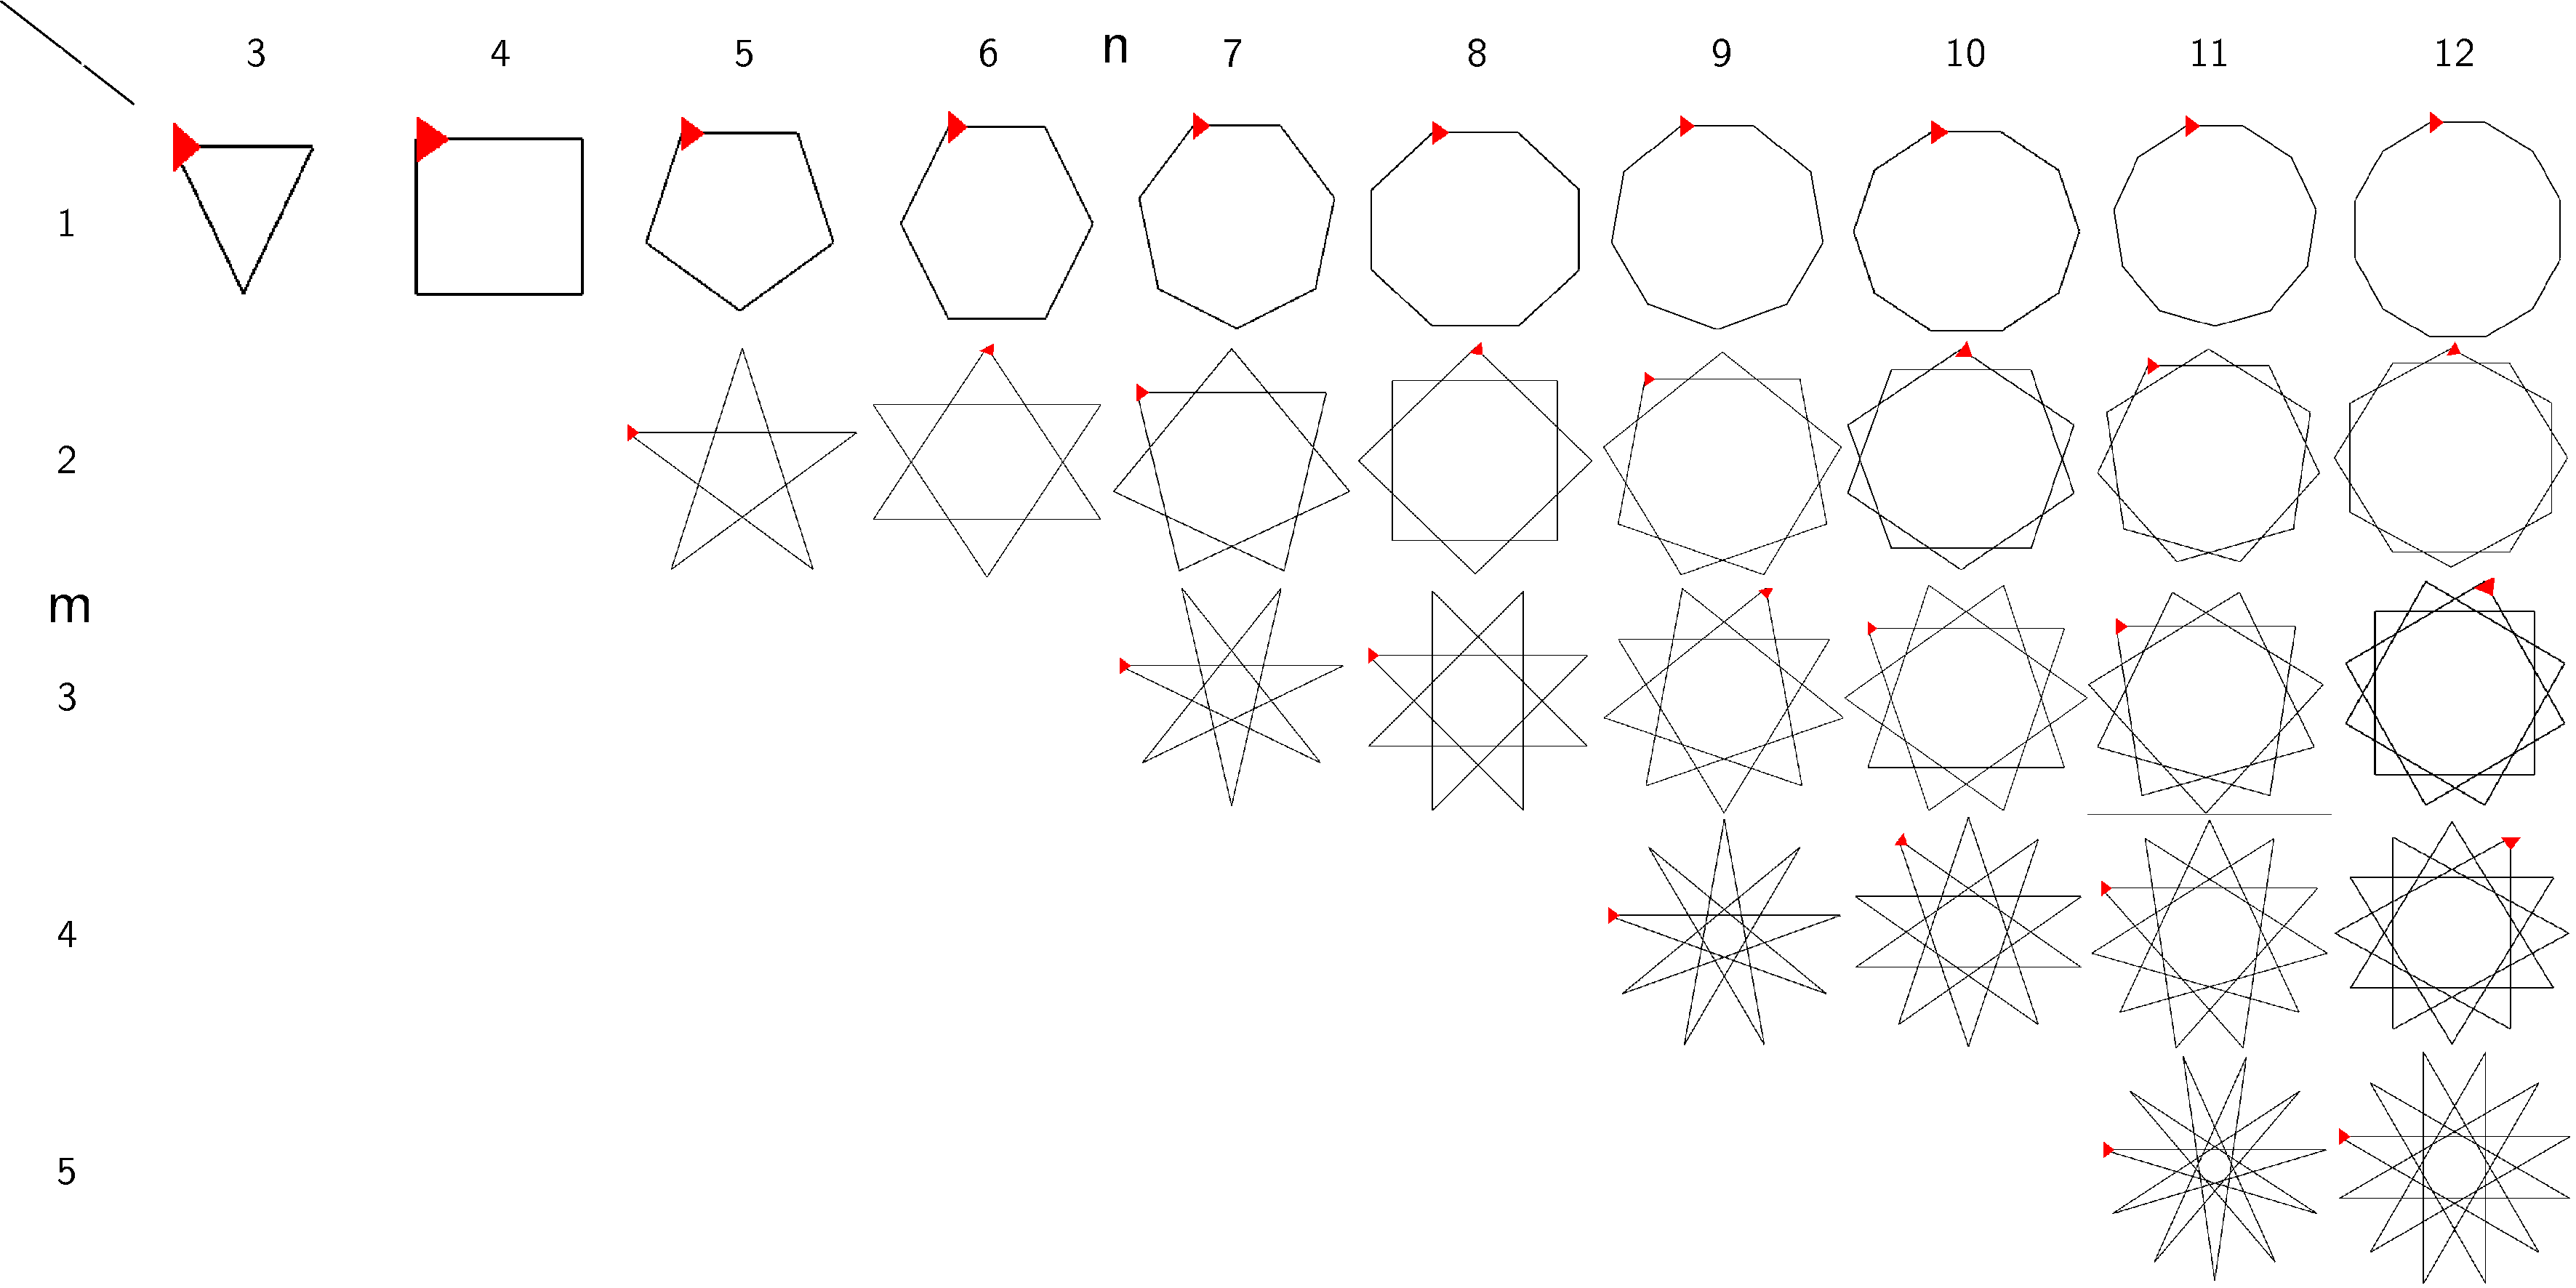
\includegraphics[width = \linewidth]{Regular Star Polygon.pdf}
	\caption{Some inputs $m,n$ and their corresponding star polygons in a tabular fashion.}
	\label{fig:regularstarpolygon}
	\end{figure}
	}
	{https://github.com/paramrathour/CS-101/tree/main/Starter Codes/Regular Star Polygon.cpp}
\end{testcasesFunction}
\begin{funvideo}
\href{https://youtu.be/oEN0o9ZGmOM}{The 3-4-7 miracle. Why is this one not super famous? -- Mathologer}
\end{funvideo}
\end{document}